%%%
 %
 % Copyright (C) 2019 Ángel Iván Gladín García
 %
 % This program is free software: you can redistribute it and/or modify
 % it under the terms of the GNU General Public License as published by
 % the Free Software Foundation, either version 3 of the License, or
 % (at your option) any later version.
 %
 % This program is distributed in the hope that it will be useful,
 % but WITHOUT ANY WARRANTY; without even the implied warranty of
 % MERCHANTABILITY or FITNESS FOR A PARTICULAR PURPOSE.  See the
 % GNU General Public License for more details.
 %
 % You should have received a copy of the GNU General Public License
 % along with this program.  If not, see <http://www.gnu.org/licenses/>.
%%%

%%%%%%%%%%%%%%%%%%%%%%%%%%%%%%%%%%%%%%%%%%%%%%%%%%%%%%%%%%%%%%%%%%%%%%%%%%%%%%%%%%%%%%%%%
\documentclass[12pt,letterpaper]{article}
\usepackage[margin=.6in]{geometry}
\usepackage[utf8]{inputenc}
\usepackage[spanish]{babel}
\decimalpoint

\usepackage{listings}
\usepackage{color}
\usepackage{graphicx}
\usepackage{enumerate}
\usepackage{enumitem}
\usepackage{float}

\usepackage{longtable}
\usepackage{hyperref}
\usepackage{commath}

\usepackage{bbm}
\usepackage{dsfont}
\usepackage{mathrsfs}
\usepackage{amsmath,amsthm,amssymb}
\usepackage{mathtools}
\usepackage{longtable}

%%%%%%%%%%%%%%%%%%%%%%%%%%%%%%%%%%%%%%%%%%%%%%%%%%%%%%%%%%%%%%%%%%%%%%%%%%%%%%%%%%%%%%%%%%%%%%%%5

\usepackage{import}

\usepackage[utf8]{inputenc}

\usepackage{listings}
\usepackage{color}

\definecolor{codegreen}{rgb}{0,0.6,0}
\definecolor{codegray}{rgb}{0.5,0.5,0.5}
\definecolor{codepurple}{rgb}{0.58,0,0.82}
\definecolor{backcolour}{rgb}{0.95,0.95,0.92}

\lstdefinestyle{mystyle}{
    backgroundcolor=\color{backcolour},   
    commentstyle=\color{codegreen},
    keywordstyle=\color{magenta},
    numberstyle=\tiny\color{codegray},
    stringstyle=\color{codepurple},
    basicstyle=\footnotesize,
    breakatwhitespace=false,         
    breaklines=true,                 
    captionpos=b,                    
    keepspaces=true,                 
    numbers=left,                    
    numbersep=5pt,                  
    showspaces=false,                
    showstringspaces=false,
    showtabs=false,                  
    tabsize=2
}

\lstset{style=mystyle}
%%%%%%%%%%%%%%%%%%%%%%%%%%%%%%%%%%%%%%%%%%%%%%%%%%%%%%%%%%%%%%%%%%%%%%%%%%%%%%%%%%%%%%%%%


%%%%%%%%%%%%%%%%%%%%%%%%%%%%%%%%%%%%%%%%%%%%%%%%%%%%%%%%%%%%%%%%%%%%%%%%%%%%%%%%%%%%%%%%%
\newcommand{\Z}{\mathbb{Z}}
\newcommand{\N}{\mathbb{N}}
\newcommand{\Q}{\mathbb{Q}}
\newcommand{\R}{\mathbb{R}}
\newcommand{\Pro}{\mathds{P}}
\newcommand{\Oh}{\mathcal{O}} %% Notacion "O"
\newcommand{\lra}{\longrightarrow}
\newcommand{\ra}{\rightarrow}
\newcommand{\ord}{\text{ord}}
\newcommand{\sol}{\textbf{\underline{Solución}: }} %% Solucion
\newcommand{\af}{\textbf{\underline{Afirmación}: }}
\newcommand{\cej}{\textbf{\underline{Contraejemplo}: }}

%%%%%%%%%%%%%%%%%%%%%%%%%%%%%%%%%%%%%%%%%%%%%%%%%%%%%%%%%%%%%%%%%%%%%%%%%%%%%%%%%%%%%%%%%

\begin{document}

%%%%%%%%%%%%%%%%%%%%%%%%%%%%%%%%%%%%%%%%%%%%%%%%%%%%%%%%%%%%%%%%%%%%%%%%%%%%%%%%%%%%%%%%%
\title{
        Universidad Nacional Autónoma de México\\
        Facultad de Ciencias\\
        Complejidad Computacional\\
    \vspace{1cm}
    \large
        \textbf{Tarea 4}\\
        \textbf{\textit{Multicommodity Integral Flow}}
}
\author{
    Ángel Iván Gladín García\\
    No. cuenta: 313112470\\
    \texttt{angelgladin@ciencias.unam.mx}
}
\date{4 de octubre 2019}
\maketitle
%%%%%%%%%%%%%%%%%%%%%%%%%%%%%%%%%%%%%%%%%%%%%%%%%%%%%%%%%%%%%%%%%%%%%%%%%%%%%%%%%%%%%%%%%

%%%%%%%%%%%%%%%%%%%%%%%%%%%%%%%%%%%%%%%%%%%%%%%%%%%%%%%%%%%%%%%%%%%%%%%%%%%%%%%%%%%%%%%%%
\newtheorem{theorem}{Teorema}
\newtheorem{example}{Ejemplo}
\newtheorem{corollary}{Corolario}
\newtheorem{lemma}{Lemma}
\newtheorem{definition}{Definicion}
\newtheorem{prop}{Proposicion}
%%%%%%%%%%%%%%%%%%%%%%%%%%%%%%%%%%%%%%%%%%%%%%%%%%%%%%%%%%%%%%%%%%%%%%%%%%%%%%%%%%%%%%%%%

%%%%%%%%%%%%%%%%%%%%%%%%%%%%%%%%%%%%%%%%%%%%%%%%%%%%%%%%%%%%%%%%%%%%%%%%%%%%%%%%%%%%%%%%%
Sea $G(V,E)$ una digráfica, con una función de capacidad $c(e)$ $(>0)$ definida en las aristas.
Vértices $s_1,s_2,t_1,t_2$ (no necesariamente distintos) ejercen un rol especial: $s_1$ y
$s_2$ son llamados \emph{fuentes} y $t_1$ y $t_2$ llamados \emph{sumideros}. Esta información
especifica la red.

Un flujo \textit{two commodity} en una red está definido por dos fucniones $f_1(e)$ y $f_2(e)$,
definidas en las atistas, que satifacen las siguientes condiciones:

\begin{enumerate}
    \item Para cada $e \in E$, $f_1(e) \geq 0$, $f_2(e) \geq 0$ y
    $$  f_1(e) + f_2(e) \leq c(e)  $$
    \item Para cada producto (\textit{commodity}) $i \in \{ 1,2 \}$ y cada vértive
    $v \in V \setminus \{ s_i, t_i \}$
    $$  \sum_{e \in \alpha(v)} f_i(e) = \sum_{e \in \beta(v)} f_i(e)   $$
\end{enumerate}

El flujo total $F_1$ y $F_2$, de las funciones del flujo $f_1$ y $f_2$, son definidas por:
$$  F_i = \sum_{e \in \alpha(v)} f_i(e) - \sum_{e \in \beta(v)} f_i(e)  $$

Se restringe a que $f_1(e)$ y $f_2(e)$ son enteros y se asume que $c(e)$ también lo es.

Un problema de flujo entero \textit{two-commodity} en una red dirigida (D2CIF) está
definido como:

\bigbreak

\textbf{Entrada:} Un red dirigida $N$ y dos enteros no negativos $R_1$ y $R_2$, llamados
requerimientos.

\bigbreak

\textbf{Pregunta:} ¿Hay funciones en el flujo entero $f_1$ y $f_2$ para $N$, para las
cuales $F_i \geq R_i$?

\bigbreak

Se mostrarará que D2CIF es NPC, incluso si todas las capacidades de las aristas son 1;
esto es llamado el D2CIF simple.

\begin{theorem}
D2CIF simple es NPC
\begin{proof}
    Mostremos que SAT $\propto$ D2CIF simple. La entrada $I$, de SAT, consiste en cláusulas\\
    $C_1, C_2, \ldots , C_m$, cada subconjunto del conjunto de literales
    $L = \{ x_1,x_2,\ldots, c_n, \bar{x_1}, \bar{x_2},\ldots,\bar{x_n} \}$. La estructura de
    $f(I)$, la entrada del D2CIF simple está como sigue. Para cada variable $x_i$ construimos
    un \textit{lóbulo}\footnote{No supe como traducir \textit{lobe}.} como se muestra
    en\ref{fig:10_7}. Aquí $p_i$ es el número de ocurrencias de $x_i$ in las cláusulas, y $q_i$
    es el número de ocurrencias de $\bar{x_i}$. Los lóbulos estan conectados en series:
    $v_i^i$ está conectado por una arista con $v_s^{i+1}$, $s_1$ está conectado con $v_s^1$ y
    $v_t^n$ a $t_1$, $s_2$ está conectada por aristas a todos los vértives $v_j^i$ y 
    $\bar{v_j^i}$ donde $j$ es impar. Además de esto, hay vértives $C_1, C_2, \ldots, C_m$ y
    una arista por cada una a $t_2$. Para la j-ésima ocurrencia de $x_i$ ($\bar{x_i}$), hay una
    atista de $v_{2j}^i$ ($\bar{v_{2j}^i}$) al vértice $C_r$, la cláusa en que ocurre.
    Los requerimientos son $R_1 = 1$ y $R_2 = m$.
    
    \begin{figure}
        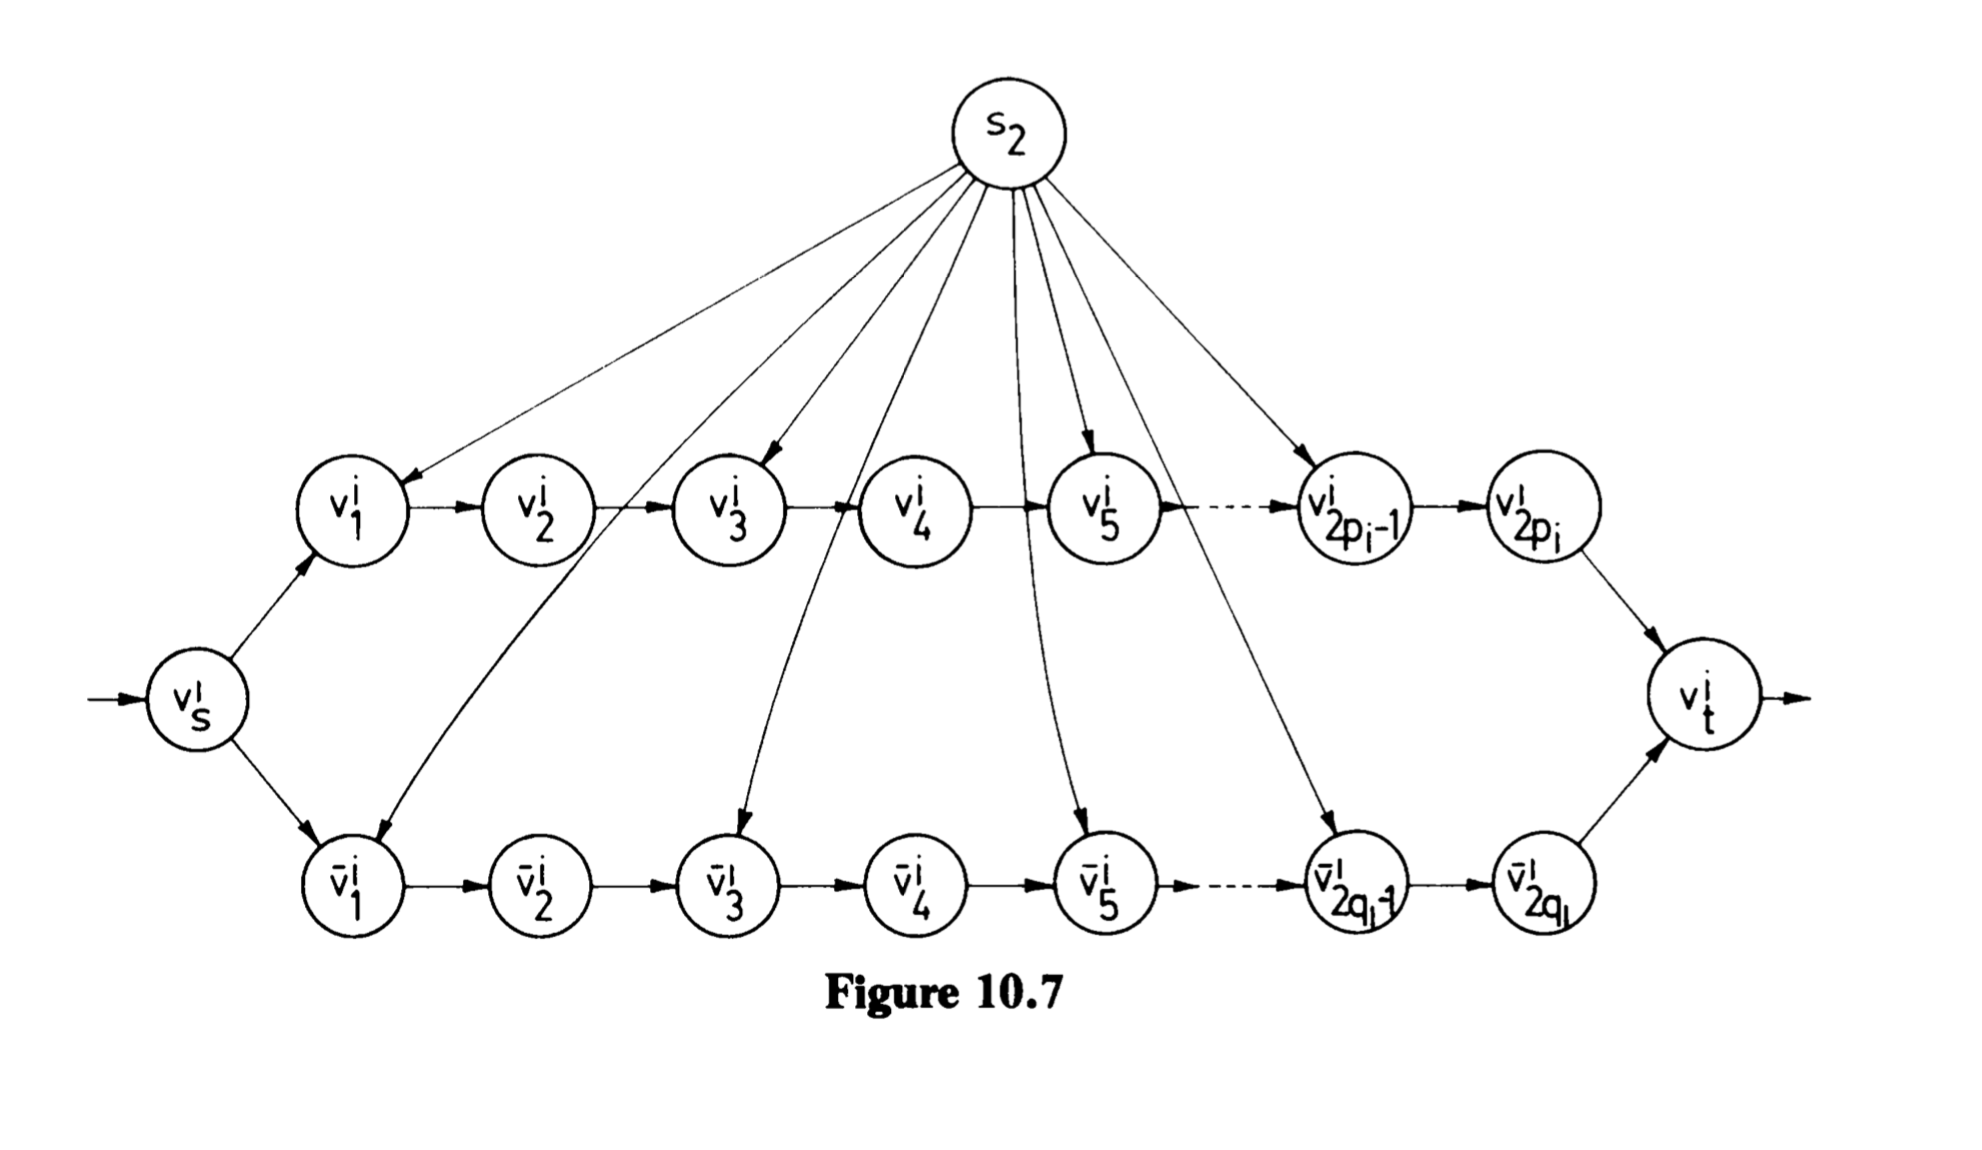
\includegraphics[scale=0.5]{assets/1.png}
        \label{fig:10_7}
    \end{figure}

    El primer producto (\textit{commodity}) debe fluir de $s_1$ a $t_1$, a través de los lóbulos;
    los vértices $s_2, C_1, C_2, \ldots, C_m$ y $t_2$ no pueden ser usados en este flujo porque
    como no hay arista del lóbulo a $s_2$, y no hay arista de regredo de $C_1, C_2, \ldots, C_m$
    y $t_2$ a los lóbulos o a $t_1$. Por tanto, la unidad del del primer producto debe usar cada 
    lóbulo o la ruta superior o inferior, pero no ambas.

    Si el segundo producto alcanza los requerimientos, entonces $F_2 = R_2 = m$, y todas las aristas
    que entrar a $t_2$ están saturadas. En este caso hay exactamente una unidad de flujo, en el
    segundo producto entrando cada $C_k$. Si esta unidad del fujo viene de una pista superior del
    i-ésimo lóbulo, a través de la arista $v_{2j}^i \to C_k$, entonces claramente usa también la
    arista $v_{2j-1}^i \to v_{2j}^i$ y la unidad del primer producto debe usar la pista de abajo 
    es ese lóbulo.

    Por tanto, si la respuesta a $f(I)$, con respecto a D2CIF, es positica, entonces podemos usar
    los flujos $f_1$ y $f_2$ para asignar una asignación satisfactora a las literales como sigue:
    Si el primer producto va a través de la pista de abajo del i-ésimo lóbulo, asignar $x_i = T$,
    y si va a través de de la superior, $x_i = F$. En este caso, la respuesta a $I$, con respecto 
    a SAT, es también positiva.

    De manera análoga, asumimos que hay una asignación satisfactoria a las variables. Si $x_i = T$,
    sea el primer producto usa la pista inferior en el i-ésimo lóbulo; si $x_i = F$, usar la
    pista superior. Ahora, sea $\xi$ sea una literal verdadera en $C_k$, Si $\xi = x_i$ entonces 
    la pista superior está libre del primer producto y podemos usar para fluir una unidad del segundo
    producto desde $s_2$ a $C_k$; si $\xi = \bar{x_i}$ entonces usar la pista inferior.
    Finalmente, usar $m$ aristas entrado $t_2$ fluir en las $m$ unidades disponibles del
    segundo producto.
\end{proof}
\end{theorem}

En el caso de las redes no dirijidas, la gráfica $G(V,E)$ es no dirigida.

El flujo en las aristas puede ser o en una dirección, y
$$  f_i(u \overset{\mathrm{e}}{-} v) = f_i(v \overset{\mathrm{e}}{-} u) $$

La condición (1) en las arista es cambiada a:
$$  | f_1(u \overset{\mathrm{e}}{-} v) + f_2(u \overset{\mathrm{e}}{-} v)| \leq c(e)$$

La condición (2), para cada $v \in V \setminus \{ s_i,t_i \}$, el flujo total del i-ésimo producto
entrando $v$ es igual al flujo total del i-ésimo producto emanando de $v$, es ahora en la
siguiente forma:

$$  \sum_{u \overset{\mathrm{e}}{-} v \in E} f_i(u \overset{\mathrm{e}}{-} v) = 0   $$

Notar que en esta ecuación $v$ está fijada. Claramente,
$$  F_i = \sum_{u \overset{\mathrm{e}}{-} v \in E} f_i(u \overset{\mathrm{e}}{-} t_i)   $$

El flujo entero no dirigido \emph{two-commodity} (U2CIF) es definido similarmente a D2CIF.

\bigbreak

\textbf{Entrada:} Una red no dirigida $N$ con dos enteros no negativos $R_1$ y $R_2$.

\bigbreak

\textbf{Pregunta:} ¿Hay funciones en un flujo entero $f_1$ y $f_2$ para $N$, tal que $F_i \geq R_i$?

\begin{theorem}
    U2CIF simple es NPC.
\end{theorem}
%%%%%%%%%%%%%%%%%%%%%%%%%%%%%%%%%%%%%%%%%%%%%%%%%%%%%%%%%%%%%%%%%%%%%%%%%%%%%%%%%%%%%%%%%



%%%%%%%%%%%%%%%%%%%%%%%%%%%%%%%%%%%%%%%%%%%%%%%%%%%%%%%%%%%%%%%%%%%%%%%%%%%%%%%%%%%%%%%%%
\begin{thebibliography}{}

    \bibitem{}
    Even, S. (2011). Graph Algorithms (G. Even, Ed.). Cambridge: Cambridge University Press.
    
    doi:10.1017/CBO9781139015165

\end{thebibliography}
%%%%%%%%%%%%%%%%%%%%%%%%%%%%%%%%%%%%%%%%%%%%%%%%%%%%%%%%%%%%%%%%%%%%%%%%%%%%%%%%%%%%%%%%%

\end{document}